\section{Treść Projektu}

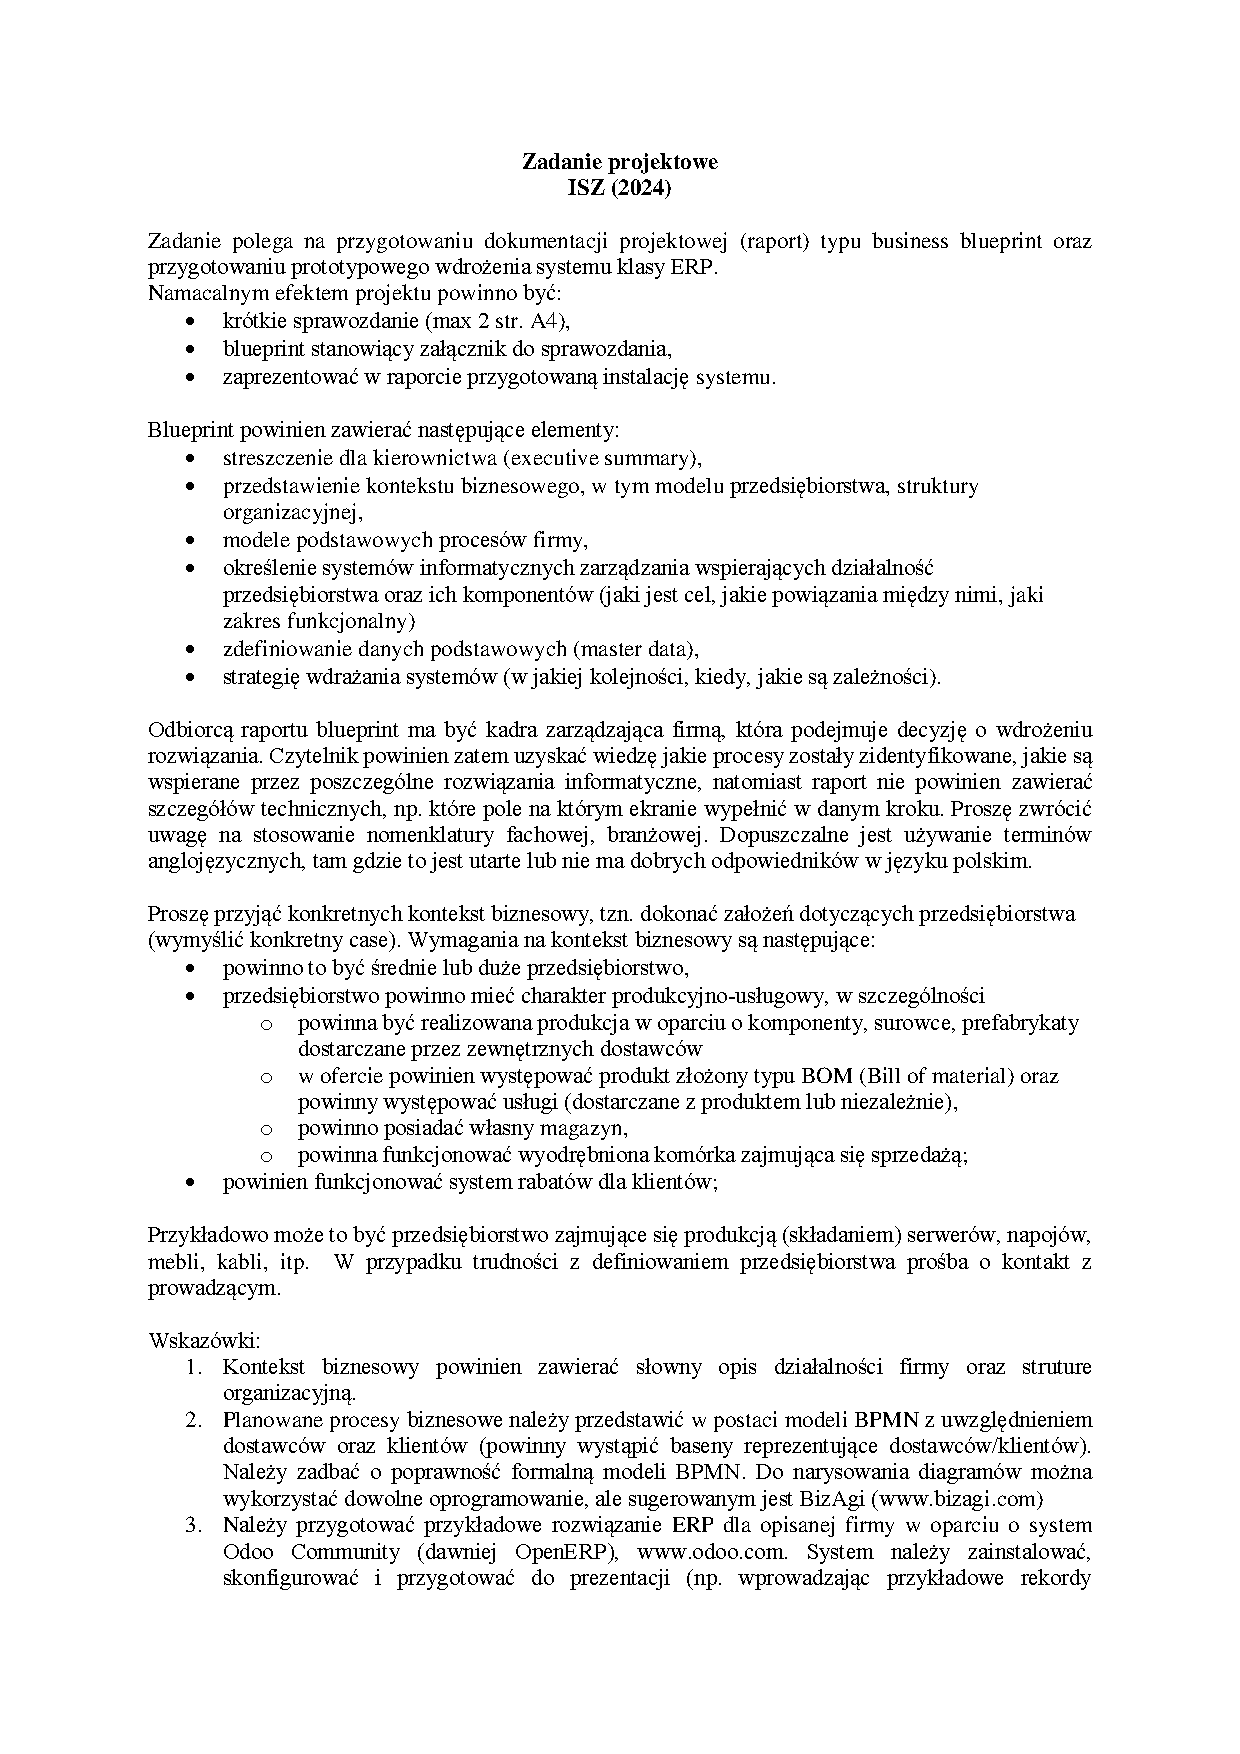
\includegraphics[width=0.9\textwidth]{tresc.pdf}\\[0.5cm]

\section{Sprawozdanie}

\subsection{Wprowadzenie}

Projekt polegał na przygotowaniu dokumentacji projektowej typu business blueprint oraz prototypowego wdrożenia systemu klasy ERP dla średniego przedsiębiorstwa produkcyjno-usługowego. W ramach projektu stworzono szereg modeli i diagramów, przeprowadzono konfigurację systemu Odoo Community, oraz zrealizowano zadanie optymalizacji procesu biznesowego.

\subsection{Przegląd działań projektowych}

Organizacja i modele procesów:
Przygotowano modele podstawowych procesów biznesowych firmy, zdefiniowano dane podstawowe oraz strategię wdrażania systemów. Modele te stworzone zostały za pomocą narzędzia Bizagi\citep{bizagi}, co umożliwiło dokładne odwzorowanie procesów z uwzględnieniem dostawców i klientów.

Instalacja i konfiguracja ERP:
System Odoo Community\citep{odoo} został zainstalowany, skonfigurowany i przygotowany do prezentacji. Wprowadzono przykładowe rekordy produktów, klientów oraz dokumentów, które ukazują różne aspekty funkcjonowania systemu. Proces konfiguracji był realizowany współbieżnie z projektowaniem procesów biznesowych, co pozwoliło na bieżące dostosowywanie systemu do potrzeb przedsiębiorstwa.

Optymalizacja procesu biznesowego:
Wybrany fragment procesu biznesowego został zoptymalizowany za pomocą języka notacji Prolog GNU Math\cite{glpk}. Model przetestowano na stronie internetowej glpk 
oraz w narzędziu GNU MathProg, co umożliwiło sprawdzenie poprawności modelu i znalezienie optymalnych rozwiązań.

\subsection{Refleksja dotycząca pozyskanej wiedzy i umiejętności}

Rozszerzenie wiedzy i umiejętności:
Projekt pozwolił na znaczne poszerzenie wiedzy z zakresu projektowania systemów ERP oraz modelowania procesów biznesowych. Dzięki pracy z Odoo Community\cite{odoo} zdobyto praktyczne umiejętności związane z konfiguracją i wdrażaniem systemów ERP. Dodatkowo, wykorzystanie narzędzia Bizagi do tworzenia diagramów BPMN przyczyniło się do lepszego zrozumienia i wizualizacji procesów biznesowych.

Materiały bazowe:
Bazą do realizacji projektu były wykłady z przedmiotu „Wspomaganie decyzji” oraz dokumentacja dostępna na stronach internetowych, takich jak dokumentacja oprogramowania Odoo. Ponadto, wykorzystano materiały dotyczące języka AMPL oraz narzędzia GNU MathProg, co umożliwiło przeprowadzenie optymalizacji procesów.

Wnioski:
Zrealizowany projekt pokazał, jak istotne jest kompleksowe podejście do wdrażania systemów ERP, obejmujące zarówno modelowanie procesów biznesowych, jak i praktyczną konfigurację systemu. Pozyskana wiedza i umiejętności z zakresu narzędzi takich jak Odoo, Bizagi oraz AMPL stanowią cenne doświadczenie, które można wykorzystać w przyszłych projektach związanych z optymalizacją i wdrażaniem systemów informatycznych w przedsiębiorstwach.

\subsection{Podsumowanie}

Projekt ISZ (2024) zakończył się sukcesem, student otrzymał niemalże maksymalną ilość punktów osiągając wszystkie zakładane cele.
 Stworzono dokumentację typu business blueprint, przeprowadzono konfigurację systemu ERP, oraz zrealizowano zadanie optymalizacji procesu biznesowego.
  Zdobyte doświadczenia i wiedza przyczynią się do dalszego rozwoju umiejętności w zakresie zarządzania procesami biznesowymi i wdrażania systemów informatycznych oraz nowe technologie i narzędzia pomocne w wprowadzeniu firmy.

